\begin{figure*}[t]
    \centering
    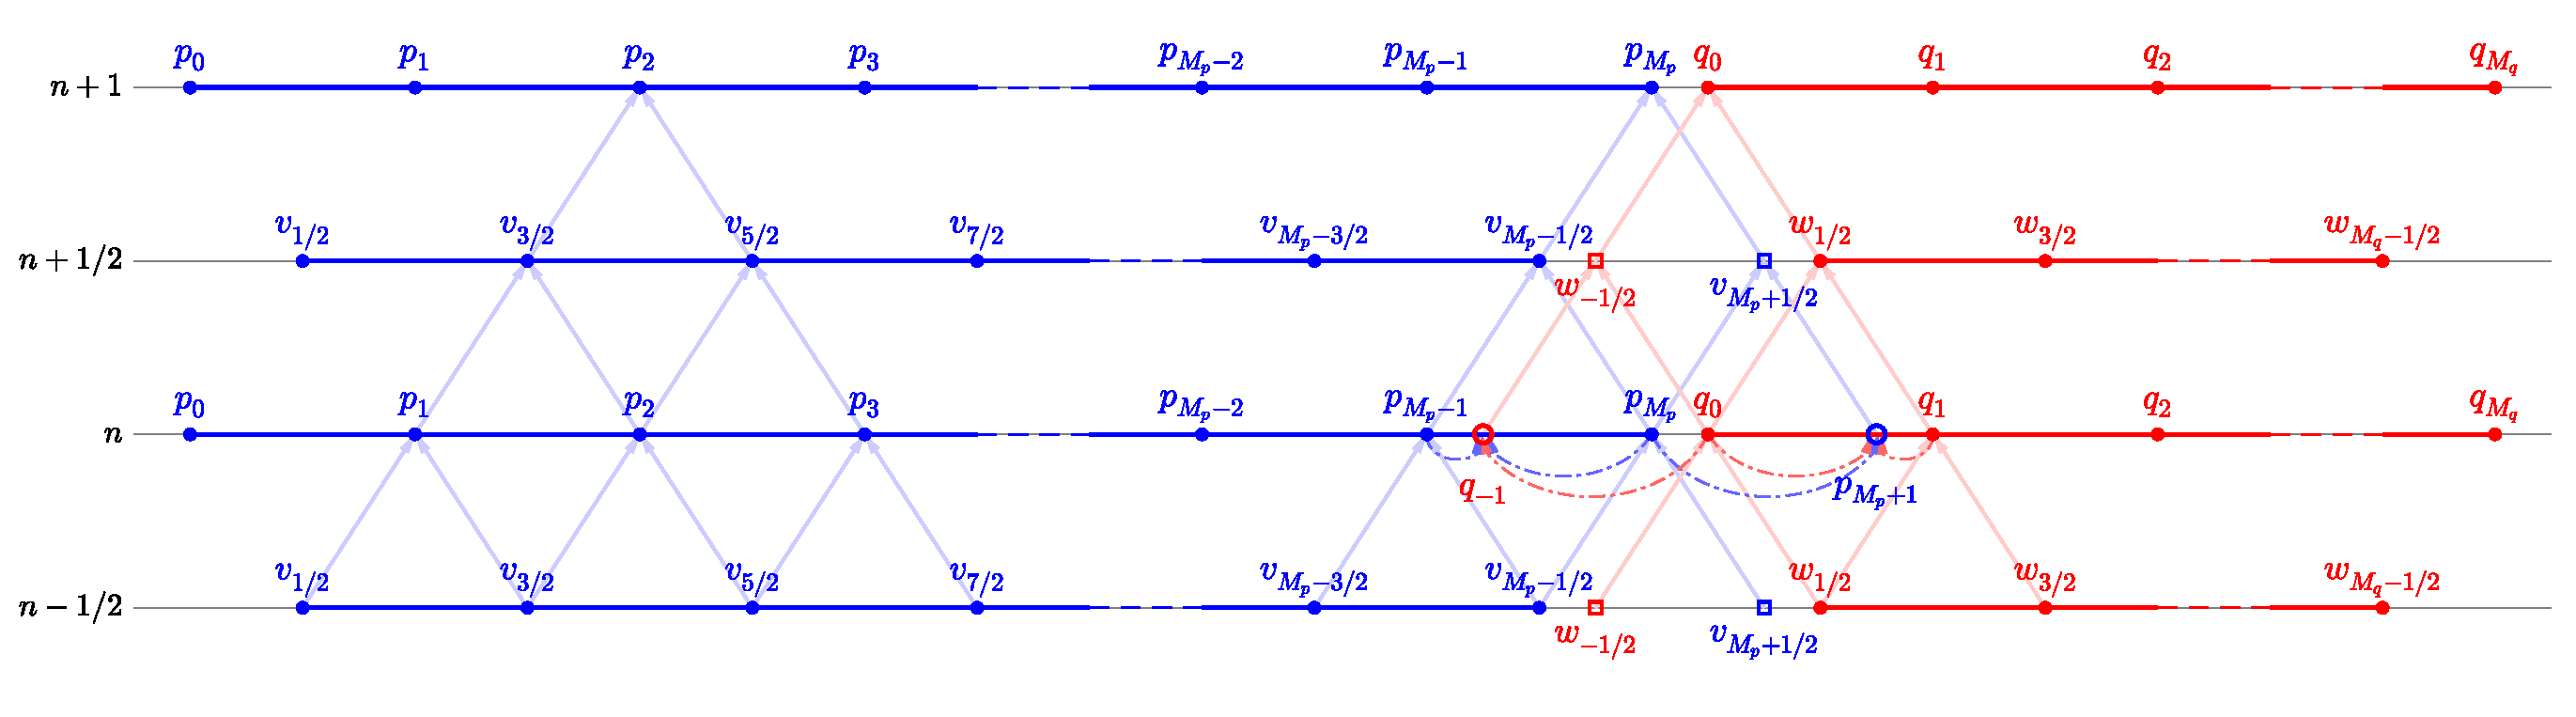
\includegraphics[width = \textwidth]{Figures/tromboneSchematic.eps}
    \caption{Schematic showing data flow of how different grid points at time index $n+1$ are calculated. To prevent cluttering, arrows going straight up (indicating that the state of a grid point at time step $n$ is needed to calculate the state of that grid point at $n+1$) are suppressed. As an example of the usual case, the points required to calculate $p_2^{n+1}$ are shown. Furthermore, the points needed to calculate $p_{M}^{n+1}$ and $q_0^{n+1}$ are shown. The most important difference with the usual case is that the virtual grid points $p_{M_p+1}^n$ %and $w_{-1/2}^n$ 
    are the result of the interpolation of known pressure values at $n$ %and velocity values at $n+1/2$ respectively
    %
    .
    %\SWcomment[Seemingly, $q_0^n$ is not calculated from anything, but it is simply $q_0^{n+1}$ time-shifted back. The same would be shown for $v_{M_p+1/2}^{n-1/2}$, but the figure does not go back-in-time more than this.]
    \label{fig:dynamicGridSchematic}}
\end{figure*}

\section{Dynamic grid}\label{sec:dynamicGrid}
Arguably the most characteristic feature of the trombone is its slide with which the length of the tube is altered and the resonating frequencies are changed. In a companion article \cite{Willemsen2021}, we present a method to dynamically change grid configurations of FDSs by adding and subtracting grid points based on paramters describing the system.

Though the paper shows changes in the wavespeed $c$ rather than the length $L$, the effect of a change in either of these parameters has an identical effect on the system \SWcomment[as long as the geometry is unchanged for the grid points.]

We can split the FDS shown in \eqref{eq:FDS} into two sets of first-order systems with lengths $L_p$ and $L_q$. The pressure and particle velocity of the left system $p_\lp^n$ and $v_{\lp+1/2}^{n+1/2}$ are defined over discrete domains $\lp = [0, \hdots, M]$ and $\lp = [0, \hdots, M-1]$ respectively. Here, $M = \lceil L_p/h\rceil$ where $\lceil \cdot \rceil$ denotes the ceiling operation. The pressure and particle velocity of the right system $q_\lq^n$ and $w_{\lq+1/2}^{n+1/2}$ are defined over discrete domains $\lq = [0, \hdots, M_q]$ and $\lq = [0, \hdots, M_q-1]$ respectively. Here $M_q = \lfloor L_q/h\rfloor$ where $\lfloor \cdot \rfloor$ denotes the flooring operation. The resulting system then becomes
\begin{subequations}
    \begin{align}
        \frac{\bar S_\lg}{\rho_0 c^2}\delta_{t+}p_\lp^n &= -\delta_{x-}(S_{\lg+1/2}v_{\lp+1/2}^{n+1/2}),\label{eq:discPressureP}\\
        \rho_0 \delta_{t-}v_{\lp+1/2}^{n+1/2}&=-\delta_{x+}p_\lp^n,\label{eq:discVelocityV}\\
        \frac{\bar S_\lg}{\rho_0 c^2}\delta_{t+}q_\lq^n &= -\delta_{x-}(S_{\lg+1/2}w_{\lq+1/2}^{n+1/2}),\label{eq:discPressureP}\\
        \rho_0 \delta_{t-}w_{\lq+1/2}^{n+1/2}&=-\delta_{x+}q_\lq^n,\label{eq:discVelocityV}
    \end{align}
\end{subequations}
The outer boundaries of this system, i.e., $\lp = 0$ and $\lq = M_q$, are the same as for the full system. The inner boundaries, $\lp = M$ and $\lq = 0$, however, are connected according to the method described in \cite{Willemsen2021} which will briefly be explained below. To calculate $p_M^{n+1}$ and $q_0^{n+1}$, points outside of their respective domains seem to be needed, i.e., $v_{M+1/2}$ and $w_{-1/2}$ which in their turn need $p_{M+1}$ and $q_{-1}$. In \cite{Willemsen2021} we propose to calculate these \textit{virtual grid points} based on known values of the system. Despite the fact that \cite{Willemsen2021} applies the method to a second-order system, it can still be applied here. A visual of how the inner boundaries are calculated can be found in Figure \ref{fig:dynamicGridSchematic}.

We start by introducing a fractional number of intervals $\Nfrac$, which is essentially Eq. \eqref{eq:numberOfIntervals} without the flooring operation (so $N = \lfloor \Nfrac \rfloor$). The fractional part of $\Nfrac$ can then be calculated using
\begin{equation}
    \alpha = \alpha^n = \Nfrac^n - N^n,
\end{equation}
which essentially describes
which can be used 
Quadratic Lagrangian interpolation is used to calculate $p_{M+1}^n$ and $q_{-1}^n$ according to
\begin{subequations}\label{eq:connectionInterpol}
\begin{align}
        &p_{M+1}^n = \frac{\alpha - 1}{\alpha + 1}p_{M}^n + q_0^n - \frac{\alpha - 1}{\alpha + 1}q_1^n
    \label{eq:calcPMp1}\\
        &q_{-1}^n
        =-\frac{\alpha - 1}{\alpha + 1}p_{M-1}^n + p_{M}^n+ \frac{\alpha - 1}{\alpha + 1}q_{0}^n.\label{eq:calcQm1}
\end{align}
\end{subequations}
which can then be used to calculate $v_{M+1/2}^{n+1/2}$ and $w_{-1/2}^{n+1/2}$ and consequently $p_M^{n+1}$ and $q_0^{n+1}$. This process repeats every sample. 





One can change the 


As the geometry varies it matters a lot where points are added and subtracted. 


\subsection{Adding and removing grid points}
Use average to prevent drift when $\alpha = 0$ and stays 0.

The main challenge, though, is to apply the method to a system of first-order equations rather than the second-order 1D wave equation presented in \cite{Willemsen2021}. \SWcomment[Rather than adding points to the left and right system in alternating fashion, points are added to pressures $p$ and $q$ and velocities $v$ and $w$ respectively]